\section{Specifications}
\label{sec:Specifications}

\newcounter{rulei}[subsection]
\newcommand{\rcnii}{\stepcounter{rulei}\arabic{section}.\arabic{subsection}.\arabic{rulei}}
\renewcommand{\labelenumi}{\rcnii}

\subsection{Markers}
\label{sub:markers}
The arena, tokens, slots, and robots involved in the game are labelled with \textit{libkoki} markers.
Each marker pattern encodes a number.
Each marker number is associated with a particular feature within the arena, and also has an associated size.
The marker numbers and sizes are as follows:

\begin{center}
  \begin{tabular}{lcc}
    \toprule
    \textbf{Item} & \textbf{Marker Numbers} & \textbf{Marker Size (mm)} \\
    \midrule
    Arena boundary & {} 0 -- 27 & 250 \\
    Robots & 28 -- 31 & 100 \\
    Slots & 32 -- 39 & 160 \\
    Token Top & 40 -- 43 & 160 \\
    Token Bottom & 44 -- 47 & 160 \\
    Token Side & 48 -- 51 & 160 \\
    \bottomrule
  \end{tabular}
\end{center}

Two sets of marker codes will be used: one for development purpose, and one for the competition itself.
The competition set is only to be used inside the Student Robotics arena at the Student Robotics competition.
This is so that people carrying markers past the arena do not confuse robots.
The competition codes are 100 above the development codes.
When run in competition mode (specifiable through the robot's GUI), the software provided by Student Robotics will subtract 100 from the detected marker codes, as well as ignore the development codes.

The markers can be printed on a black-and-white printer.
Marker designs can be downloaded from the documentation section of the Student Robotics website.

Unless specified otherwise, all markers described in this document are oriented vertically such that the principle corner of the marker (which is indicated by a dark grey dot in the black marker border) is on the higher edge.

\subsection{Robot Badges}
\label{sec:robot-badges}

\begin{figure}
  \centering
  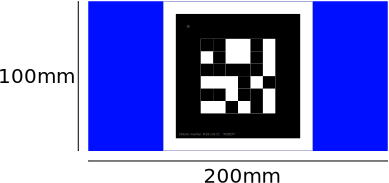
\includegraphics[width=\textwidth]{./images/robot-marker.pdf}
  \caption{An example robot badge.
           The blue areas shown are the human-compatible areas.
	   All dimensions are in millimetres.}
  \label{fig:example-badge}
\end{figure}

\begin{enumerate}
\item A ``robot badge'' is a removable identifier that will be attached to a robot throughout a match.
      It features the robot's assigned marker for the match, as well as human-compatible areas to allow spectators to easily associate a robot with its starting location.
      An example of one of these badges is shown in figure~\ref{fig:example-badge}.
      The markings in the human-compatible areas are intentionally not specified.

\item A robot must feature four of the badge mounts shown in figure~\ref{fig:badge-mounting}.
      These mounts must permit a flat $200 \times 100mm$ panel to be attached to them.
      The three areas of each mount must feature the illustrated areas of hook-type Velcro to allow this panel to be fitted.

\item The four badge mounts must be on the exterior of the robot, parallel with the vertical plane, and should be perpendicular to each other about the vertical axis\footnote{Teams can apply for a team-specific rule alteration to the required number of badges.
      Clear justification must be provided by the team with such a request.}
      The orientation of the badge mounts is unimportant, but teams are encouraged to position them horizontally as shown in figure~\ref{fig:example-badge}.

\item The mapping between a given robot and its robot badge is as follows:

\begin{center}
  \begin{tabular}{cc}
    \toprule
    \textbf{Corner} & \textbf{Marker Number} \\
    \midrule
    0 & 28 \\
    1 & 29 \\
    2 & 30 \\
    3 & 31 \\
    \bottomrule
  \end{tabular}
\end{center}

\begin{figure}
  \centering
  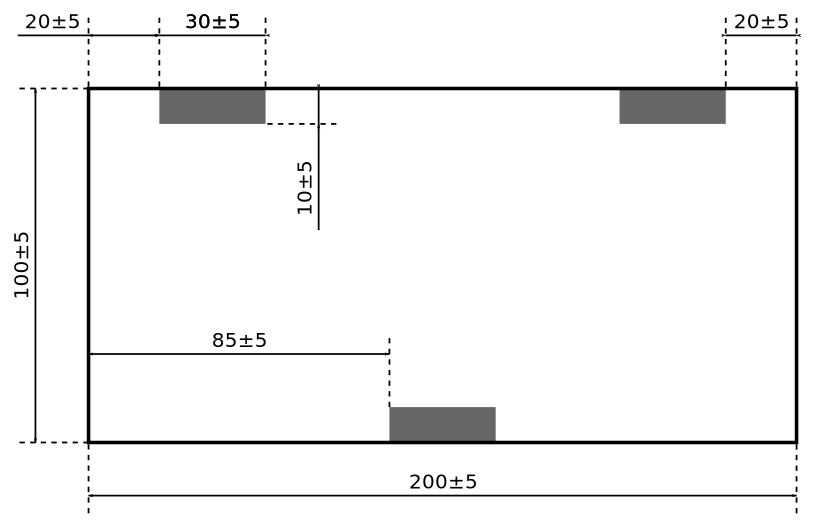
\includegraphics[width=\textwidth]{./images/badge-mounting.pdf}
  \caption{The dimensions of the required robot badge mountings.
           The shaded areas are hook-type Velcro.
           All dimensions are in millimetres.}
  \label{fig:badge-mounting}
\end{figure}

\end{enumerate}

\subsection{Arena}
\label{sub:arena}
\begin{enumerate}
\item The match arena floor, overall, is an $8m \times 8m$ square, as shown in figure~\ref{fig:arena-dim}.
      The tolerance of these two dimensions is $\pm0.25m$.

\begin{figure}
  \centering
  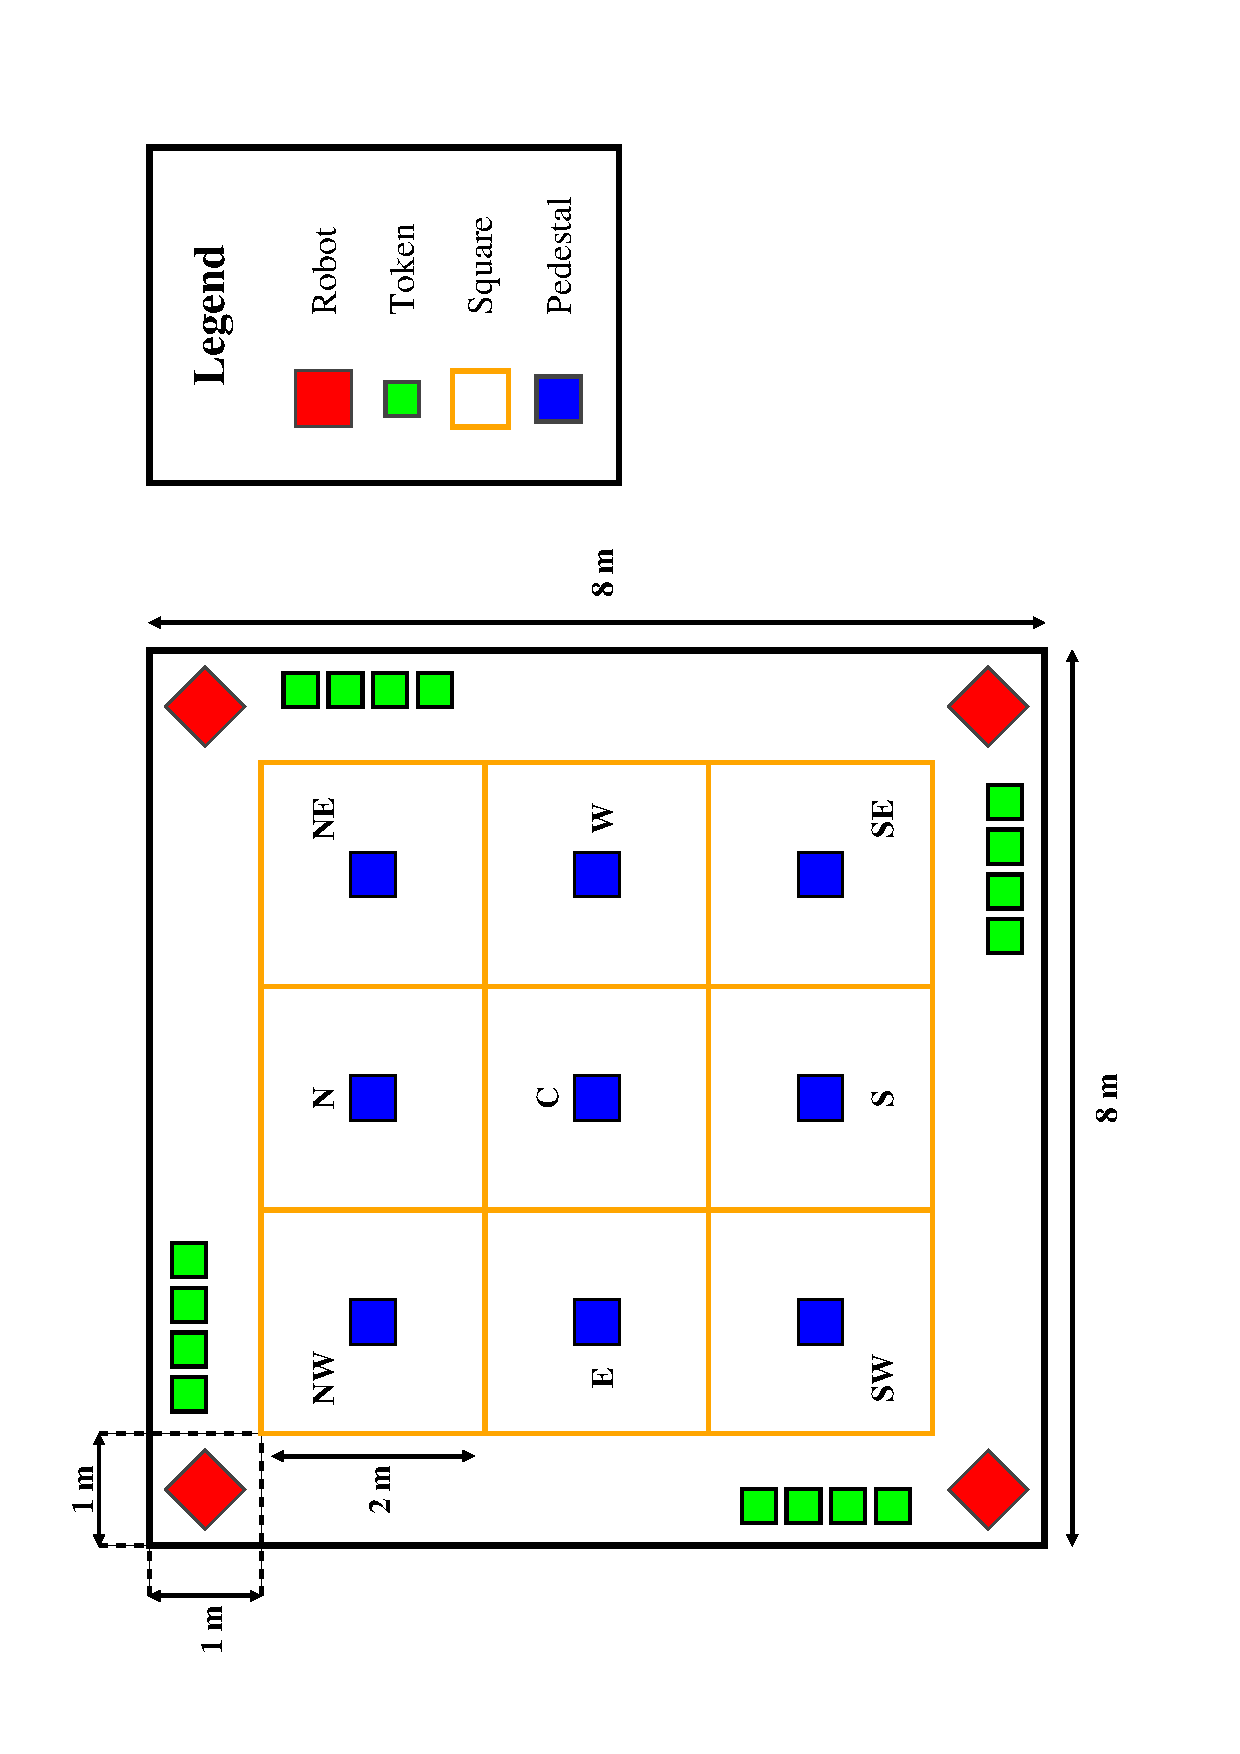
\includegraphics[width=\textwidth]{./images/arena.pdf}
  \caption{\label{fig:arena-dim}A bird's-eye view of the arena. All dimensions are in millimetres.}
\end{figure}

\item The floor of the arena is covered with a closed-loop, short pile carpet.

\item The perimeter of the arena floor is delimited by the arena wall, which has a minimum height of $100mm$.

\begin{figure}
  \centering
  
\includegraphics[width=\textwidth]{./images/sidewall.pdf}
  \caption{Seven $250mm$ wide markers are spaced evenly along each $8m$ arena wall.
           The markers are placed $50mm$ above the floor.
	   All dimensions are in millimetres.}
  \label{fig:arena-wall}
\end{figure}

\begin{figure}
  \centering
  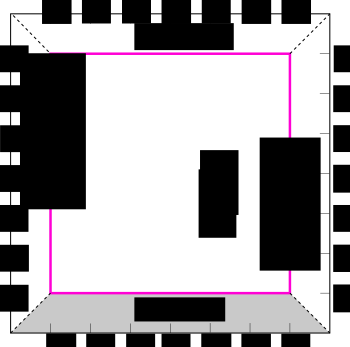
\includegraphics[width=0.5\textwidth]{./images/arena-markers.pdf}
  \caption{Twenty eight arena wall markers are positioned around the perimeter of the arena with the marker codes incrementing in a clockwise fashion.
           Eight slot markers are incremented from number 32, in an anti-clockwise fashion around the zones.
           The corners are counted in a clockwise fashion, with corner 0 being the corner closest to arena marker 0.}
  \label{fig:arena-zones}
\end{figure}

\item Each wall of the arena features seven $250mm$ libkoki markers.
      Figure~\ref{fig:arena-wall} shows the positioning of these markers, whilst figure~\ref{fig:arena-zones} shows the numbering of these markers.

\item Each robot will be assigned a corner at the start of every match to indicate its starting position.
      Corner starting positions are $1000 \pm 20mm$ square and will be marked by $25mm$ paper-based masking tape.
      The mapping of these corner numbers in the arena is shown in figure~\ref{fig:arena-zones}.

\item Student Robotics reserves the right to have up to three match officials in the arena during games.

\end{enumerate}


\subsection{Scoring Zones \& Barriers}
\label{sub:Zones}

\begin{enumerate}
\item There are four zones in the arena, each in front of one of the corners.
      The arrangement and dimensions of these zones can be seen in figure~\ref{fig:arena-dim}.

\item Part of the boundary between adjacent zones will be formed by a barrier.
      The barriers will be $100 \pm 20mm$ high, $300 \pm 20mm$ wide and $1500 \pm 20mm$ long.
      The locations of the barriers can be seen in figure~\ref{fig:arena-dim}.

\item Where the boundary of a scoring zone is not formed by either a barrier or the arena wall
      it will be marked by $25mm$ paper-based masking tape.
\end{enumerate}

\subsection{Tokens}
\label{sub:Tokens}
\begin{enumerate}
\item Tokens are wooden cubes with a side length of $250 \pm 10 mm$.

\item The overall weight of each token will be $1 \pm 0.2 kg$.

\item Tokens will be mounted on casters.
      The lower edge of each vertical face will have a ground clearance of $10 \pm 5 mm$.

\item Each token will be assigned a unique $250mm$ libkoki marker.
      This marker will be displayed on all four vertical faces of a given token.

\item Token markers are oriented such that the top left corner of each marker (identified by a small grey dot) is affixed to the top left of a token's side face.

\item The top face of each token may be adorned with a flag or another human-identifiable object to help with match commentary.
      Any such addition will not impede access to any of the four vertical faces of a token.
      Adornments will contribute to a token's overall weight.

\item There will be 5 tokens in the arena.
      Their starting positions can be seen in figure~\ref{fig:arena-dim}.

\end{enumerate}

\clearpage
